%   % !TEX root = ../../VIII,3_Rahmen-TeX_8-1.tex
%  
%   Band VIII, 3		Rubrik STOSS
%
%   Signatur/Tex-Datei:	LH_35_10_16_007
%
%   RK-Nr. 	60127		
%
%   Überschrift: 	(keine)
%   
%   Unterrubrik:			DCC Plus
%
%   edlabels:			2
%
%   Diagramme: 		2
%
%
%   NB: 						(Anmerkungen)					??
%
%
%
\selectlanguage{ngerman}
\frenchspacing
%
\begin{ledgroupsized}[r]{120mm}
\footnotesize
\pstart
\noindent\textbf{Überlieferung:}
\pend
\end{ledgroupsized}
%
\begin{ledgroupsized}[r]{114mm}
\footnotesize
\pstart \parindent -6mm
\makebox[6mm][l]{\textit{L}}%
Notiz: LH XXXV 10, 16 Bl.~7.
Ein Zettel (\phantom)\hspace*{-1.5mm}\,9,5 x 12 cm\phantom(\hspace*{-1.2mm});
oberer Rand abgerissen, die übrigen beschnitten.
Eine halbe Seite auf Bl.~7~r\textsuperscript{o};
auf Bl.~7~ v\textsuperscript{o} Kostenaufstellung von fremder Hand:
\newline
\protect\begin{tabular}{lrr}
&89&13\\
40 penning a 5 duit per gulden&2&16\\
provisie a 2 StSt per gulden&8&19\\
Vragt en bestellen pakken&-&18\\ \cline{2-3}
&fl 102&6\\
\protect\end{tabular}
\pend
\end{ledgroupsized}
%
%
\vspace{5mm}
\begin{ledgroup}
\footnotesize
\pstart
\noindent%
\textbf{Datierungsgründe:}
Die inhaltliche Auseinandersetzung mit dem Stoß sowie die Kostenaufstellung auf Holländisch sprechen für eine frühe Entstehung des Textes wahrscheinlich noch auf Leibnizens Rückreise aus Frankreich, die vom 12. bis Ende November 1676 durch die Niederlande führte.%
\protect\index{Ortsregister}{Frankreich (Gallia, Francia)}%
\protect\index{Ortsregister}{Niederlande}
\pend 
\end{ledgroup}
%
%
\selectlanguage{latin}
\frenchspacing
% \newpage%
\count\Bfootins=1000%
\count\Afootins=1200%
\count\Cfootins=1000
\vspace{8mm}
\pstart%
\normalsize%
\noindent%
\lbrack7~r\textsuperscript{o}\rbrack\
Si in Globum majorem quiescentem%
\protect\index{Sachverzeichnis}{globus major}%
\protect\index{Sachverzeichnis}{globus quiescens}
%
\edtext{\lbrack\textit{a}\rbrack}{%
\lemma{\textit{A}}\Bfootnote{%
\textit{erg.~L, ändert Hrsg.}}}
%
ingruat
%
\edtext{directe}{%
\lemma{directe}\Bfootnote{%
\textit{erg.~L}}}
%
minor,%
\protect\index{Sachverzeichnis}{globus minor}
lex haec.%
\protect\index{Sachverzeichnis}{lex concursus}
%
Sit major 1, minor $1:n,$
fiet reflexio minoris $n-1,\, :\,,\, n+1,$%
\protect\index{Sachverzeichnis}{reflexio corporis minoris}
progressus majoris $2:\,,n+1.$%
\protect\index{Sachverzeichnis}{progressus corporis majoris}%
%%%% ACHTUNG: Mit der Cfootnote getrixt.
\edtext{}{%
\lemma{\hspace{1,6mm}\lbrack\textit{Fig.~1}\rbrack}\killnumber\Cfootnote{%
Das Diagramm zeigt vermutlich zwei mögliche Stoßrichtungen.%
}}%
\pend
%
%
\vspace{1.5em}
\centerline{\hspace{70mm}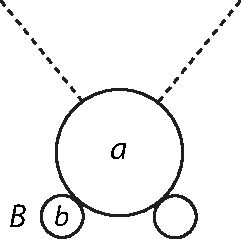
\includegraphics[width=0.18\textwidth]{gesamttex/edit_VIII,3/images/LH_35_10_16_007_d1_007r.pdf}}%
\vspace{0.5em}
\centerline{\hspace{70mm}\lbrack\textit{Fig.~1}\rbrack}%
\vspace{-9.2em}
%\newpage
%
%
%\vspace{0.5em}
\pstart
$\begin{array}{c||c|c} a & v & x \\ b & y & z \end{array}$%
\pend
\vspace{0.5em}
%
\pstart
\noindent
$a(v-x)=bz$
\quad
\edlabel{35_10_16_007_1a}%
$v+x=z$%
\edtext{}{%
{\xxref{35_10_16_007_1a}{35_10_16_007_1b}}%
{\lemma{$v+x=z$}\Bfootnote{%
\textit{(1)}~$v=z-x=bz+ax$
\textit{(2)}~$av-ax=bv+bx$%
~\textit{L}}}}%
\pend
%
\pstart
\noindent
$av-ax=bv+bx$,%
\edlabel{35_10_16_007_1b}
%
\quad
et
$x=v,\, a-b,\, :\,,\, a+b$ %
\pend
%
\pstart
\noindent
$a(2v-z)=bz,$
\quad
fit
$z=v,\, 2a :\,,\, a+b$ %
\pend
%
\pstart
\noindent
$x:z=a-b,\, :\,,\, 2a$
\pend
\newpage
%
\pstart
Si globus \textit{a}%
\protect\index{Sachverzeichnis}{globus major}
incidat directe in globum quiescentem \textit{b}%
\protect\index{Sachverzeichnis}{globus minor}%
\protect\index{Sachverzeichnis}{globus quiescens}
erit celeritas globi \textit{a} nova%
\protect\index{Sachverzeichnis}{celeritas globi nova}
ad priorem%
\protect\index{Sachverzeichnis}{celeritas globi prior}
ut $a-b$ ad
%
\edlabel{35_10_16_007_2a}%
$a+b$.
\edtext{}{%
{\xxref{35_10_16_007_2a}{35_10_16_007_2b}}%
{\lemma{$a+b.$}\Bfootnote{%
\textit{(1)}~Si corpus
\textit{(2)}~Si globus major
\textit{(a)}~\textit{A}
\textit{(b)}~\textit{a} ingruat in mino
\textit{(3)}~Si globus
\textit{(a)}~\textit{A}
\textit{(b)}~\textit{a} motus, incidat indirecte in globum \textit{b}%
~\textit{L}}}}%
%
\pend
%
\pstart
Si globus \textit{a} motus, incidat indirecte in globum \textit{b}%
\edlabel{35_10_16_007_2b}
%
quiescentem
\lbrack\textit{Text bricht ab.}\rbrack
\pend
%
\vspace{2.0em}
\centerline{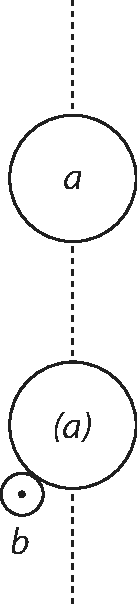
\includegraphics[width=0.09\textwidth]{gesamttex/edit_VIII,3/images/LH_35_10_16_007_d2_007r.pdf}}
\vspace{0.5em}
\centerline{\lbrack\textit{Fig.~2}\rbrack}
\count\Bfootins=1200%
\count\Afootins=1200%
\count\Cfootins=1200
%\vspace{0.5em}
%
%
%
%    %    %    %    Ende des Textes auf Bl. 7r
